\newpage
\subsection{Salinization}
Salinization is the increase of salt concentration in soil and is, in most cases, caused by dissolved salts in the water supply. This supply of water can be caused by flooding of the land by seawater, seepage of seawater or brackish groundwater through the soil from below.

In April of 2016, a report has been made on the drought and salinity intrusion in the Mekong River Delta of Vietnam. It concluded that the salinity intrusion has worsened due to climate change and drought. It is useful to take a closer look at this report. \cite{salinity}

\subsubsection{The cause of salinity}
Salinity intrusion in the Mekong Delta is heavily caused by low water discharge from upstream of the Mekong River. Lesser rain falls in the Mekong basin lead to a reduction in upstream water flow to push back seawater. The situation worsens when there is drought and high temperatures in the region.

An oscillating warming and cooling pattern, referred to as the ENSO cycle, directly affects rainfall distribution in the Mekong Delta. El Niño and La Niña are the extreme phases of the ENSO cycle.

Recently, local authorities and farmers alike underestimated the drought and salinity intrusion conditions, thus rendered them unprepared for the impacts on aquaculture and agricultural production. Rice production, a main agricultural activity, was reduced in affected areas due to salinity intrusion, lack of freshwater and drought. 

\begin{figure}[h]
\centering
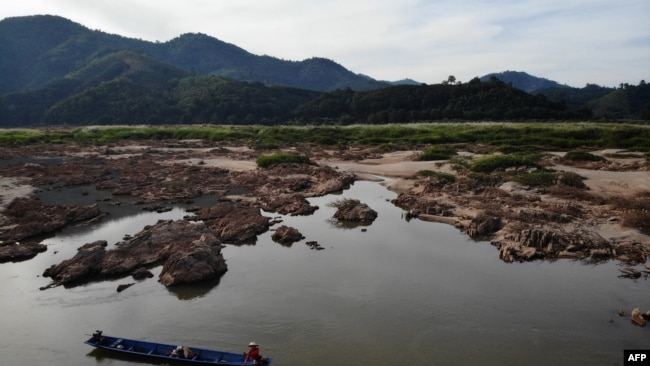
\includegraphics[scale=0.45]{mekong/12_drought.jpg}
\caption{A paddy field is hit by salinity in Mekong Delta 
\cite{saigononline}}
\end{figure}

These issues were largely caused by the below average rainfall in the Mekong basin due to the El Niño, as well as the use of hydropower dams. With insufficient upstream water flow to push back seawater, salinity intrusion increased in concentration and duration. This affected largely small-scale farmers and producers who have lower financial and technical capabilities to adapt to climate changes.

\subsubsection{Mitigation}

The Mekong Delta is heavily dependent on other countries and the climate for the flow of the Mekong River. Because of these uncontrollable dependencies, the Vietnam government opted for diversification. Shrimp farming was established along the coast, while farmers further inland started combining rice farming with freshwater aquaculture, mostly farming tilapia. Thanks to this development, Vietnam has grown into a significant exporter of shrimps and tilapia. \cite{wyrdykes}